\chapter{Startup}
\label{sec:startup} 

In this section, the first steps are described to run the application, create a database or access an existing one, import data and start the management GUI.

\section{Running the Application}

To run the application, simply execute it.

For an AppImage, use e.g.:
\begin{verbatim}
$ ./ATSDB-vX.X.X_x86_64.AppImage
\end{verbatim}

For a self-built application, use e.g.:
\begin{verbatim}
$ ./build/bin/atsdb_client
\end{verbatim}

It is recommended to run the application from a console terminal (for issue analysis of the log text), but that is not mandatory.

\section{Configuration Upgrade}

If a previous version of ATSDB has been run on the workstation, the configuration (and additional application data) might be out of date. Since the framework of ATSDB is quite sensitive on being run with the latest configuration an upgrade must be performed. \\


\includegraphics[width=0.5cm]{../../data/icons/hint.png} Please note that this means that the previous configuration will be overwritten, which will unfortunately clear any previous changes made by the user. \\\\

If an outdated configuration is detected, a dialog will be shown.

\begin{figure}[H]
    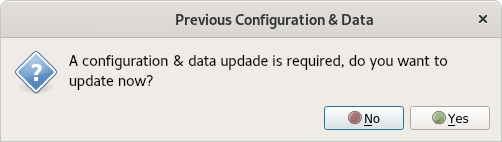
\includegraphics[width=12cm,frame]{../screenshots/config_data_update.png}
  \caption{Configuration and data update}
  \label{fig:db_connect}
\end{figure}

If 'Yes' is selected, the update is performed and the application starts. If 'No' is selected, the application will quit. If previous changes to an outdated configuration are if strong importance, please contact the author for support. 

\subfile{startup_dialog}

\subfile{startup_use_cases}

\subfile{startup_mysql_connect}
\subfile{startup_mysql_open_db}
\subfile{startup_mysql_import}

\subfile{startup_sqlite3_open}

\subfile{startup_schema_select}
\subfile{startup_manage_dbo}

\subfile{startup_import_asterix}
\subfile{startup_import_json}

\subfile{startup_datasources}

\subfile{startup_radar_pos}

\subfile{startup_artas_assoc}

\subfile{startup_starting}
